#import "@local/bootlin:0.1.0": *

#import "@local/bootlin-yocto:0.1.0": *

#import "@local/bootlin-utils:0.1.0": *

#import "../../typst/local/themeBootlin.typ": *

#import "../../typst/local/common.typ": *

#show: bootlin-theme.with( aspect-ratio: "16-9", config-common(handout: "handout" in sys.inputs and sys.inputs.handout == "1", ))

#show raw.where(block: true): set block(fill: luma(240), inset: 1em, radius: 0.5em, width: 100\%)

#show raw.where(block: true): set text(size: 11pt)

#show raw.where(block: false): r => text(fill: color-link)[#r]

#show raw.where(lang: "c", block: true): set block(fill: luma(240), inset: 0.4em, radius: 0.5em, width: 95\%, breakable: true, above: 12pt, below: 12pt)

#show raw.where(lang: "c", block: true): set text(11pt)

#show raw.where(lang: "console", block: true):set block(fill: luma(240), inset: 0.4em, radius: 0.5em, width: 95\%, breakable: true, above: 6pt)

#show raw.where(lang:"console", block: true): set text(12pt)

 = Principles

=== Set your goals

#columns(gutter: 8pt)[
    \begin{itemize}
	\item Reducing boot time implies measuring boot time!
	\item You will have to choose reference events at which you
	      start and stop counting time.
	\item What you choose will depend on the goal you want to
              achieve. Here are typical cases:
	\begin{itemize}
		\item Showing a splash screen or an animation, playing a sound to
	              indicate the board is booting
		\item Starting a listening service to handle a particular
	              message
	        \item Being fully functional as fast as possible
	\end{itemize}
    \end{itemize}
     #colbreak()
    % From https://openclipart.org/detail/46075/stop-watch-by-klaasvangend
    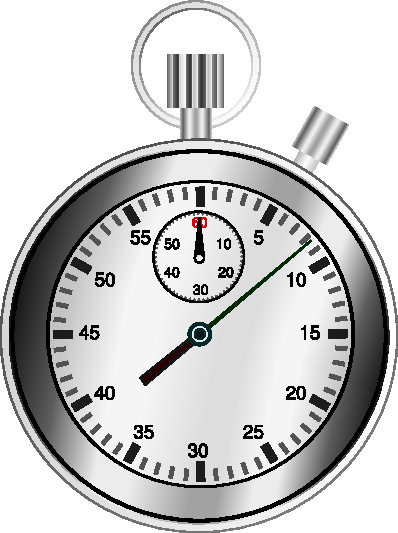
\includegraphics[width=\textwidth]{slides/boot-time-principles/stop-watch.pdf}
  \\]


=== Boot time reduction methodology
\begin{center}
    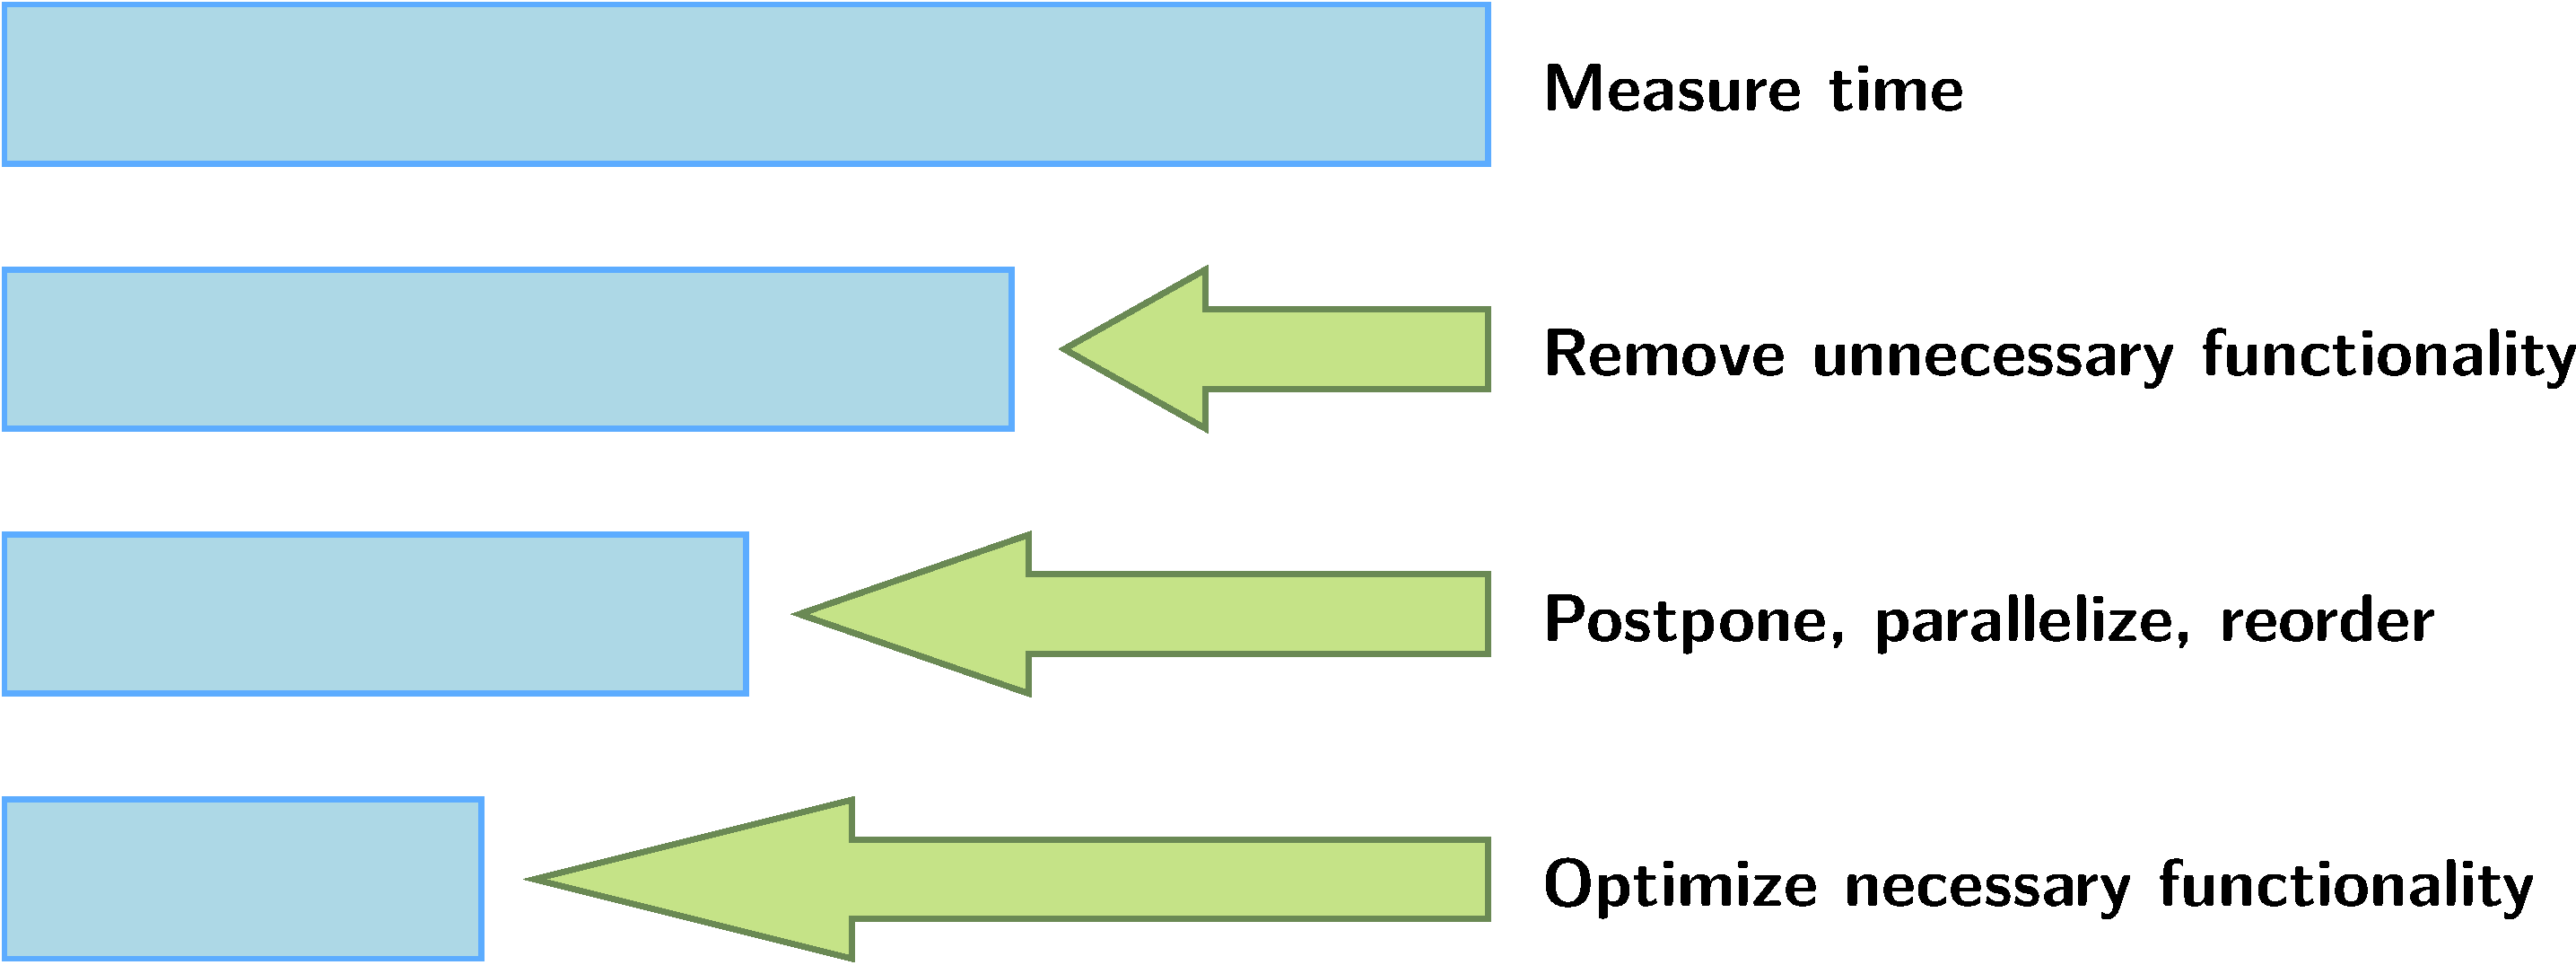
\includegraphics[width=\textwidth]{slides/boot-time-principles/methodology.pdf}
\end{center}


=== Boot time components
\begin{center}
    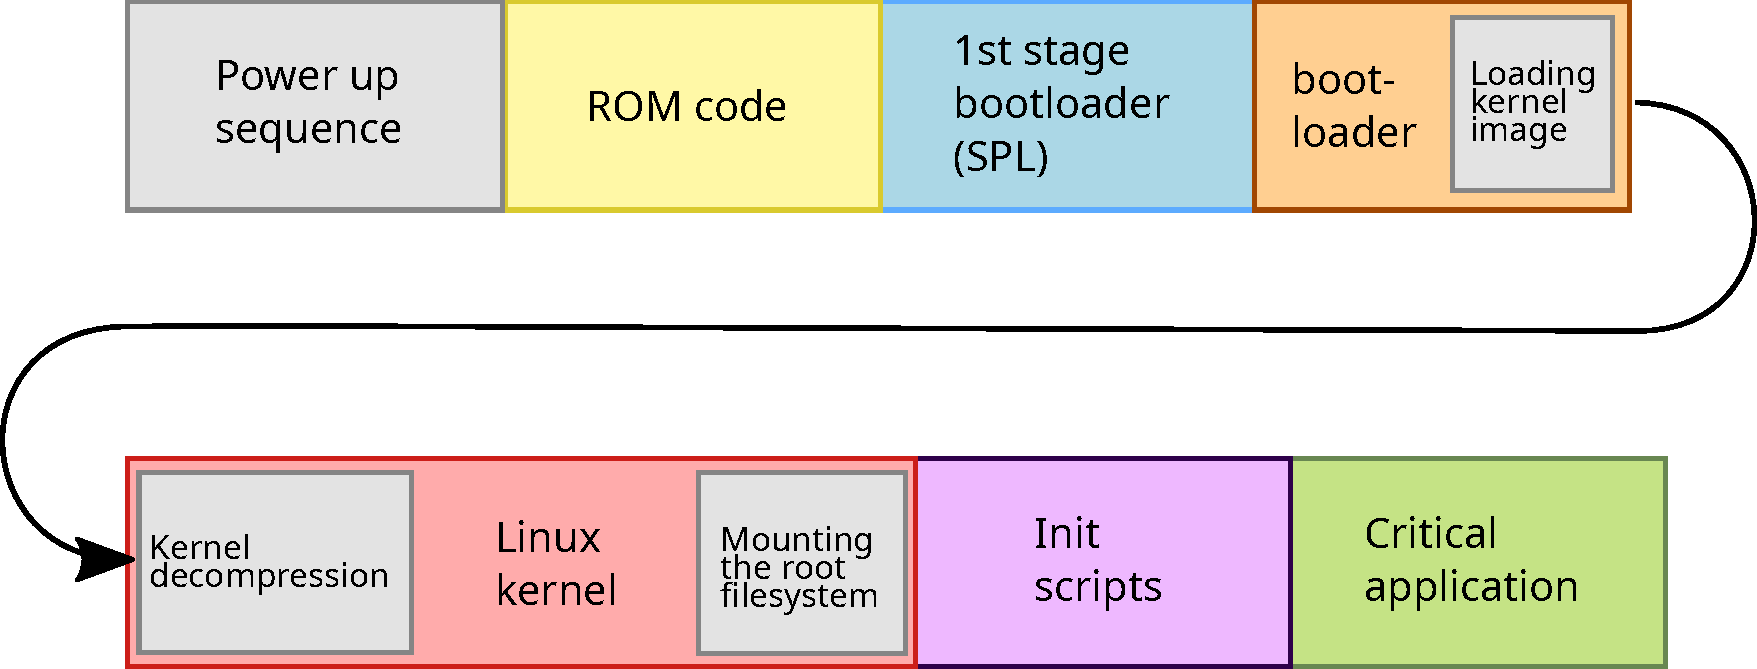
\includegraphics[width=\textwidth]{slides/boot-time-principles/generic-boot-sequence.pdf}
\end{center}
We are focusing on reducing {\em cold} boot time, from power on to the critical application.


\input{booting-process-omap.tex}

=== What to optimize first Start by optimizing the {\bf last steps} of the boot process!
\begin{itemize}
\item Don't start by optimizing things that will reduce your ability to
      make measurements and implement other optimizations.
\item Start by optimizing your applications and startup
      scripts first.
\item You can then simplify BusyBox, reducing the number of available
      commands.
\item The next thing to do is simplify and optimize the kernel. This
      will make you lose debugging and development capabilities,
      but this is fine as user space has already been simplified.
\item The last thing to do is implement bootloader optimizations,
      when kernel optimizations are over and when the kernel command
      line is frozen.
\end{itemize}
We will follow this order during the practical labs.


=== Worst things first and measurement methodology
{\em Premature optimization is the root of all evil.\\
Donald Knuth}
\begin{itemize}
\item Taking the time to measure time carefully is important.
      \begin{itemize}
           \item Advice to make at least 3 measures for each
		 configuration you want to measure.
           \item Pay attention to variations between measures.
		 Measures are only valuable when there is a low
		 jitter between them.
           \item Keep copies of all your logs. Always useful to
		 double check or analyze measures which are
                 inconsistent with the others.
      \end{itemize}
\item Find the worst consumers of time and address them first.
\item You can waste a lot of time if you start optimizing
      minor spots first.
\end{itemize}


=== Build automation
\begin{itemize}
\item Build automation is a very important part of a successful project.
\item So, through the build system, you should automate any remaining
      manual step and all the new optimizations that you will implement
      to reduce boot time. Without such automation, you may forget some
      optimizations, or introduce new bugs when making further optimizations.
\item Boot time optimization projects required countless rebuilds too,
      automating image generation will save a lot of time too.
\item Kernel and bootloader compiling and optimizations can also be
      taken care of by the build system, though the need is less critical.
\end{itemize}


=== Generic ideas Some ideas to keep in mind while trying to reduce the boot time:
\begin{itemize}
\item The fastest code is code that is not executed
\item A big part of booting is actually loading code and data from the
      storage to RAM. Reading less means booting faster. I/O are
      expensive!
\item The root filesystem may take longer to mount if it is bigger.
\item So, even code that is not executed can make your boot time
      longer.
\item Also, try to benchmark different types of storage. It has
      happened that booting from SD card was actually faster than
      booting from NAND.
\end{itemize}

